\documentclass[letterpaper, 11pt]{article}

\usepackage[letterpaper, margin=1in]{geometry}
\usepackage{indentfirst}
\usepackage{multicol}
\usepackage{graphicx}
\graphicspath{ {./} }

\begin{document}

\title{Word Embedding Informed Focused Topic Model (WEI-FTM)}
\author{Brandon Schoenfeld and Roland Laboulaye}
\date{March 13, 2018}
\maketitle

\begin{multicols}{2}

\noindent \textbf{Abstract.} Understanding the topic of a document is an easy task for humans, but
very difficult for computers.
We compare latent Dirichlet allocation (LDA), which has historically been used for topic analysis
with a recent variation, Word Embedding Informed Focused Topic Model (WEI-FTM).
WEIFTM employs a word embedding, like GloVe to capture lost semantic information and induces
sparsity on the topic models.

\section{Introduction}
From a young age, humans are trained to read and extract meaning from text.
From even just one sentence, a human can glean the topic of an author's discourse.
Computers, however, do not so readily extract meaning or even a concept for a topic as humans would
from a long sequence of binary numbers which comprise a text or document.
In fairness, a computer program which reads text has not had the same years of training as humans to
gain the ability to understand the topics contained in a document.
We explore two unsupervised learning algorithms which allow a computer to begin to group words by
topic and topics by document.

A document is an ordered collection of words and a corpus is an unordered set of documents.
Latent Dirichlet allocation[2] (LDA) models the process of generating a document, sampling
probabilistically from a distribution of words and topics.
LDA simplifies the document model by assuming that a document is a "bag-of-words", or that there is
no order to the words in a document.
While this simplifying model assumption discards information that humans consider valuable to
understanding a text, it facilitates learning topics over a corpus.

The original LDA publication[2] showed some success in task of modeling topics over
large documents with many word co-occurrences, but with few weaknesses that are strengthened by a
more recent variation on this approach.
Because each document is treated as a bag-of-words, most inter-word relationships are lost.
Also, LDA struggles to learn topics when documents are relatively short.
A lack of word co-occurrences disallows the model to learn which words go together when an author
discusses any particular topic.

Zhao, et. al.[1], proposed what they termed a Word Embedding Informed Focused Topic
Model (WEI-FTM).
Word embeddings, like GloVe[3], seek to learn a representation for words
which captures both semantic and syntactic information and facilitates numerical and machine learning
analyses on text.
WEI-FTM uses these word embeddings to enrich the topic modeling process by capturing some of the
information lost by the bag-of-words simplification.
Furthermore, word embeddings mitigate the problem of low word co-occurrences of shorter texts by
providing meaning which longer documents capture.
Additionally, while LDA modeling each topic as a distribution over all words in a vocabulary,
the WEI-FTM model allows for the possibility of removing any number of words from the distribution
for a topic.
The model can focus each topic on the words that it determines are most relevant to the topic, given
the corpus.

We present both the LDA and the WEI-FTM models in sufficient detail as well as Gibss sampling, an
algorithm which attempts to recover the latent parameters used in the generative process of the
models.
We also present a simple adaptation in the use of word embeddings which reduces dimensionality in
the word embedding space and speeds up the inferential process.
Finally, compare both of these models on corpora with short documents and long documents.

\section{LDA Model}
\subsection{Generative Model}
Latent Dirichlet allocation treats each document in a corpus of text as a "bag of words", generated
by a probabilistic model.
The generative process is as follows:
\begin{enumerate}
	\item $N \sim Poisson(\xi)$
	\item $\theta \sim Dirichlet(\alpha)$
	\item For each of the $N$ words $w_n$:
	\begin{itemize}
		\item Topic $z_n \sim Multinomial(\theta)$ 
		\item $w_n \sim p(w_n | z_n, \beta)$, a $Multinomial$
	\end{itemize}
\end{enumerate}

\noindent The following graphic demonstrates this generative process using plate notation:

\begin{center}
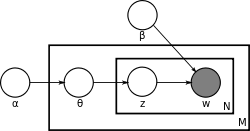
\includegraphics[scale=.75]{lda}
\end{center}

In the generative process, $\alpha$ and $\beta$ are known, but in the inference portion, they either
must be supplied by the user as hyperparameters or included in the sampling process.

\subsection{Gibbs Sampling}
The generative LDA model provides a framework for inference over a particular corpus.
For any given corpus, the parameters of the corresponding generative model, $\theta$ and $z$, are
not known and must be learned.
For simplicity in sampling, an auxiliary parameter $\phi$ is introduced to incorporate $\beta$ and
determine a distribution for topics over words.

Gibbs sampling is a Markov chain Monte Carlo (MCMC) algorithm which explores the joint probability
space over the entire model.
The probability of the model is given by:
\[
	p(W, Z, \theta, \phi, \alpha, \beta) =
\]
\[
	\prod\limits_{k=1}^{K} A(k)
	\prod\limits_{m=1}^{M} B(m)
	\prod\limits_{n=1}^{N} C(m,n)
\]
\noindent where
\[
	A(k) = p(\phi_k; \beta)
\]
\[
	B(m) = p(\theta_m; \alpha)
\]
\[
	C(m,n) = p(Z_{m,n} | \theta_m) p(W_{m,n}|\phi_{Z_{m,n}})
\]
\noindent This algorithm, for one pass or epoch, iterates over each document and each word.
It holds all parameters constant, except one, for each iteration.
A new topic is sampled for the given word and $\theta$ and $\phi$ are updated accordingly.
Because all parameters are held constant save one, this algorithm is known to run slowly.
However, a good model can often be found with few epochs, depending on the parameter initialization
and the corpus.

\section{WEI-FTM Model}
Similar LDA, the word embedding informed focused topic (WEI-FTM) model assumes a corpus was built
using a generative process.
Once again, Dirichlet priors are placed over the topic distributions under documents and over the
word distributions under topics.
Because the Dirichlet distribution is the conjugate prior of the categorical distribution, sampling
becomes much easier.
Unlike LDA, WEI-FTM takes advantage of two mechanisms to improve the sampling process and resulting
model: word embeddings, which capture semantic and syntactic information, and a focusing or
sparsity inducing of the words in each topic.

First, word embeddings are incorporated into the model using parameters $\lambda$ and $c$.
This is particularly helpful when the corpus contains short documents where word co-occurrence data
is lacking.
Word embeddings allow the model to leverage relationships between words in embedded space.
At the beginning of the generative process, $\lambda$ and $c$ are sampled from a multivariate
gaussian distribution.
$\lambda$ and $c$ are then used to apply a linear transformation to the word embeddings, with
$\lambda$ acting as a set of weights and $c$ acting as a bias.
This transformation is stored in $\pi$, a matrix of shape number of topics by vocabulary size.

The focusing mechanism is implemented in the form of a binary matrix $b$ of shape number of topics
by vocabulary size.
The $k, v$ entry $b$ indicates whether or not word $v$ is allowed to be included in the distribution
for topic $k$, with $b[k, v] = 0$ meaning that word $v$ is excluded from topic $k$.
Each entry of $b$ is sampled from a Bernoulli distribution with probability equal to the sigmoid of
the corresponding entry of $\pi$.
Since $\pi$ contains information extracted from word embeddings, the sampling of $b$ is largely
impacted by the word embeddings.
The sparsity matrix $b$ gives the model flexibility to determine which words are relevant to each
topic while completely ignoring the rest of the words in the vocabulary of the corpus.

Once $b$ has been generated, $\phi$ is sampled from a Dirichlet distribution that takes a
combination of $\beta$ and $b$ as its parameters.
Through $b$, the topic representation $\phi$ can be more focused than its counterpart in LDA.
The remainder of the generative process is identical to LDA’s.

As in LDA, while the each document in the corpus is assumed to have been created by the generative
process, the original parameters are not known and must be estimated.
Because of the conjugacy of the distributions in the WEI-FTM model, Gibbs sampling can infer the
unknown parameters with relative efficiency.
Because WEI-FTM has word embedding and focused topic components, there are additional parameters
not in the LDA model that must be estimated.
For every iteration of Gibbs Sampling, not only does a topic assignment need to be sampled for each
word in each document, but an entry from the focus-matrix $b$ must be sampled for the word, and
corresponding parameters for $\lambda$ and $c$ must be sampled as well.


\section{Reduced word embedding dimensionality with PCA}
The word embedding provides some semantic and syntactic information about each word in a very high
dimensional space.
Any particular corpus, especially the ones with which we are working, contains a very small subset of
of the words which the word embedding describes.
We conjectured that perhaps the variance of the words in the corpus within the embedding space
could be described with a more concise representation than the full embedding dimensionality.
We decided to apply Principal Component Analysis (PCA) to the subset of the word embedding which describes
the input corpus.
We used sklearn's PCA implementation, which allows the user to specify the size of the reduced
dimensionality.
Since we are working in a very high dimensional space and there can be much variability between
many corpora, we decided to dynamically choose the size of the reduced embedding space to capture
at least 97 percent of the variance in the given corpus.
Using this modification, we saw performance gains of 33-50 percent, depending on the corpus, without
any loss in the model's ability to learn topics.

\section{Evaluation}
In order to evaluate our model, we began by constructing a simple dataset, generated according to
LDA’s generative model.
We hardcoded $\theta$ and $\phi$ distributions and sampled from them using the Dirichlet
distribution in order to create 100 documents from 3 topics.
Shown below, the first graph shows the log likelihood flattening out and the second graph shows the
classification accuracy where a document’s label is defined as the argmax of its topic probability
distribution.

\begin{center}
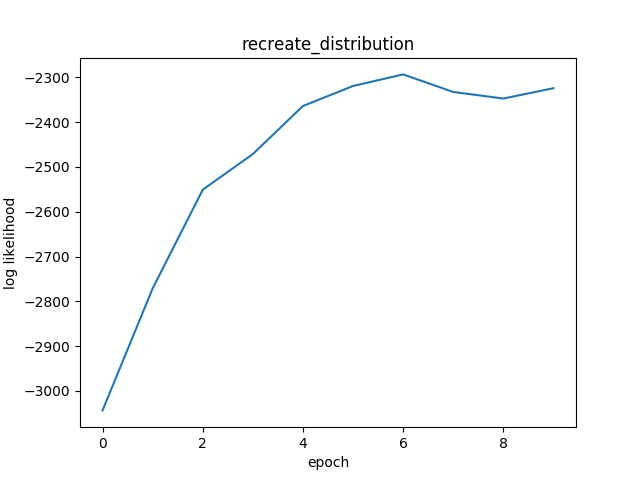
\includegraphics[scale=.3]{log_likelihood}
\end{center}

\begin{center}
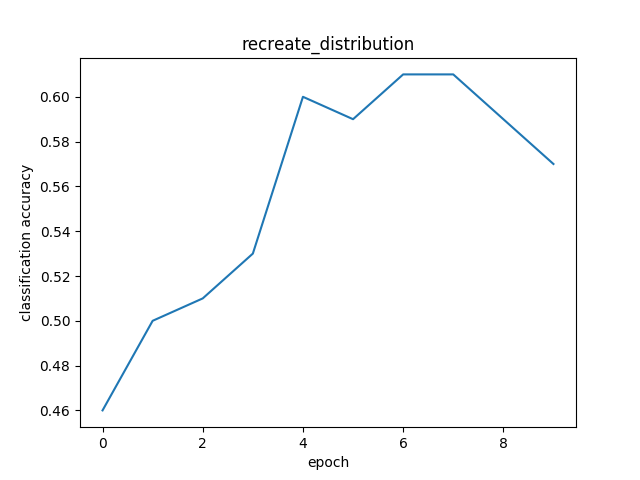
\includegraphics[scale=.3]{accuracy}
\end{center}

\noindent These plots illustrate that our WEI-FTM model was able to identify an appropriate
parameter setting for this problem and was able to far outdo the default accuracy of .33.
However, the fact that it is an unsupervised algorithm and that documents are generated through
sampling and so do not correspond perfectly to their label prevented it from reaching a very high
accuracy.

Having verified that our model worked, we thought that using text from social media would be most
appropriate as WEI-FTM is designed specifically for use on short text.
We chose a dataset of 1000 yelp reviews, 500 positive and 500 negative.
We were curious to see what topics the model would identify and whether it would be able to
recreate the classes despite its unsupervised nature.

We first report the log likelihood curves and the classification accuracy curves for our datasets
and then perform a qualitative analysis of the quality of our generated topics, while comparing
them to the topics generated by LDA.

\begin{center}
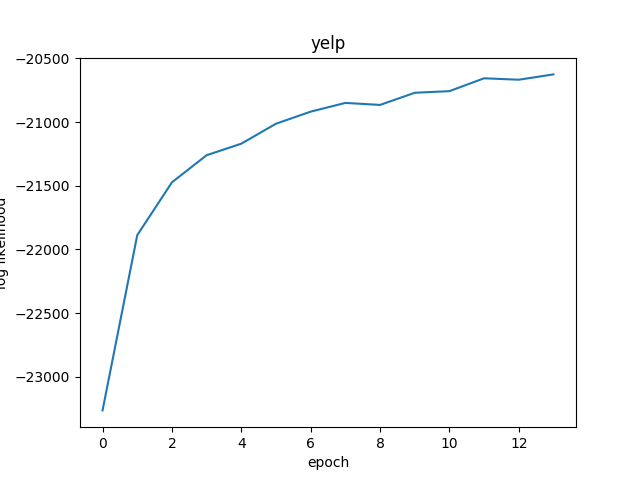
\includegraphics[scale=.3]{yelp_log_like_short}
\end{center}

\begin{center}
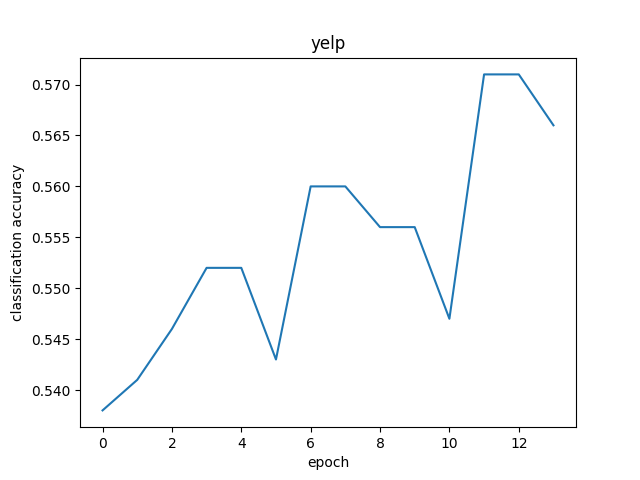
\includegraphics[scale=.3]{yelp_acc_short}
\end{center}

\begin{center}
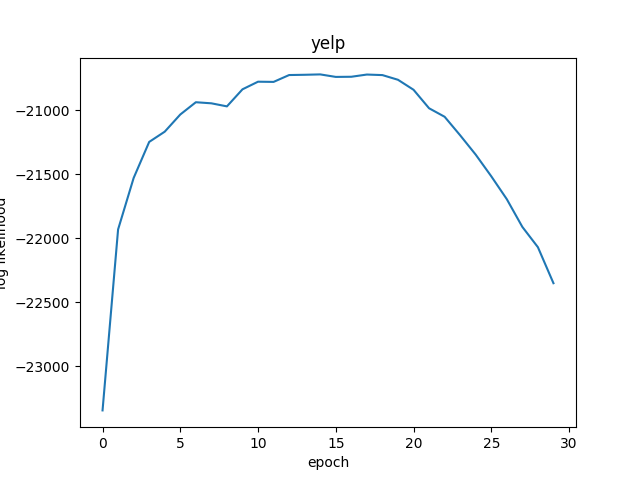
\includegraphics[scale=.3]{yelp_log_like_long}
\end{center}

\begin{center}
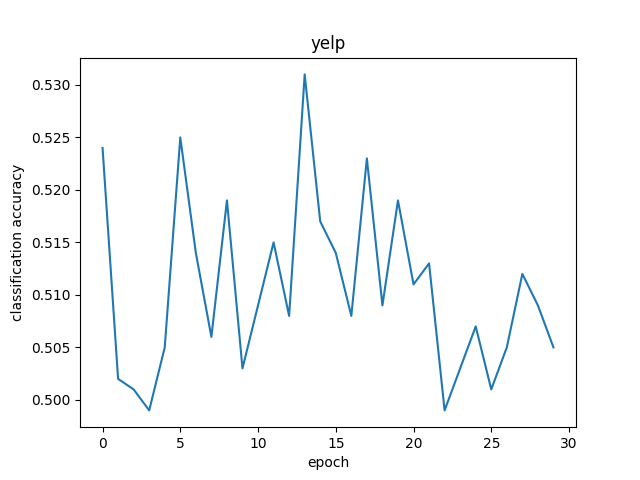
\includegraphics[scale=.3]{yelp_acc_long}
\end{center}


As shown by the first two graphs above, WEI-FTM is able to find parameter setting that allows its
log likelihood to plateau and to marginally increase its classification accuracy.
However, the lower two graphs illustrate that the model is unstable.
Even when in a stable setting, the probabilistic nature of the algorithm allow it to occasionally
explore suboptimal areas.
As such, we see our log likelihood decrease after a number of epochs.
Of interest is the fact that as the log likelihood decreases, so does the classification accuracy,
showing that the topic models generated were slightly correlated with the existing classes,
positive and negative reviews.

The highest probability words associated with the two topics (shown below) give some insight into
the topics generated by LDA and WEI-FTM for the Yelp dataset.
While neither fully captures the dichotomy between positive and negative reviews, a qualitative
evaluation reveals that, unlike LDA, the WEI-FTM representation of topic 1 has quite a few
negative words while its topic 0 has almost only positive words.
While this is only a cursory observation, it appears that WEI-FTM is better extracting topics from
short text.

\begin{center}
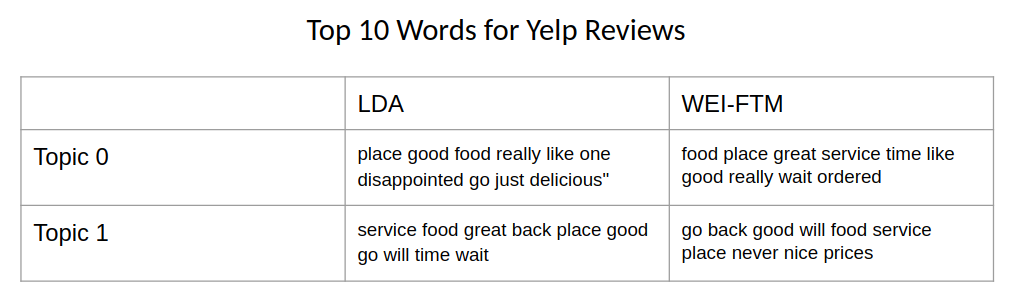
\includegraphics[scale=.23]{yelp_table}
\end{center}

\section{Conclusion}
WEI-FTM is certainly by no means a perfect answer to LDA’s shortcomings. It is slower than LDA and mostly produces similar results. However, it seems that its reliance on word embeddings does enable it to extract slightly better topic models than LDA when running on very short documents (tweets, facebook posts, etc.). For future work, it would be interesting to continue investigating ways to better align the leveraged word embeddings with the needs of the topic model instead of relying on general semantic embeddings. While our creative work in this area is promising, we think generating word embeddings specifically suited to a bag-of-words model might yield better results.

\section{Bibliography}
\begin{enumerate}
\item Zhao, H, et al. “A Word Embeddings Informed Focused Topic Model.” Proceedings of Machine Learning Research vol. 77, 2017, pp. 423–438, http://proceedings.mlr.press/v77/zhao17a/zhao17a.pdf.

\item Blei, D, et al. “Latent Dirichlet Allocation.” Journal of Machine Learning Research, vol. 3, 2003, pp. 993–1022, www.jmlr.org/papers/volume3/blei03a/blei03a.pdf.

\item Jeffrey Pennington, Richard Socher, and Christopher D. Manning. 2014. GloVe: Global Vectors for Word Representation.

\item Williamson, S, et al. “The IBP Compound Dirichlet Process and its Application to Focused Topic Modeling.” Proceedings, 27th International Conference on Machine Learning, 2010, pp. 1151–1158., www.cs.columbia.edu/~blei/papers/WilliamsonWangHellerBlei2010.pdf.

\item Geman, S. and Geman, D. “Stochastic relaxation, Gibbs distributions and the Bayesian restoration of images.” IEEE Transactions on Pattern Analysis and Machine Intelligence, vol. 6, 1984, pp. 721–741.
\end{enumerate}

\end{multicols}
\end{document}
